\chapter{Design}\label{ch:design}

In this chapter we describe the approach and design of the of the implemented solution.
First and foremost, a automatic certification process should avoid user interaction whenever possible.

\begin{figure}
    \centering
    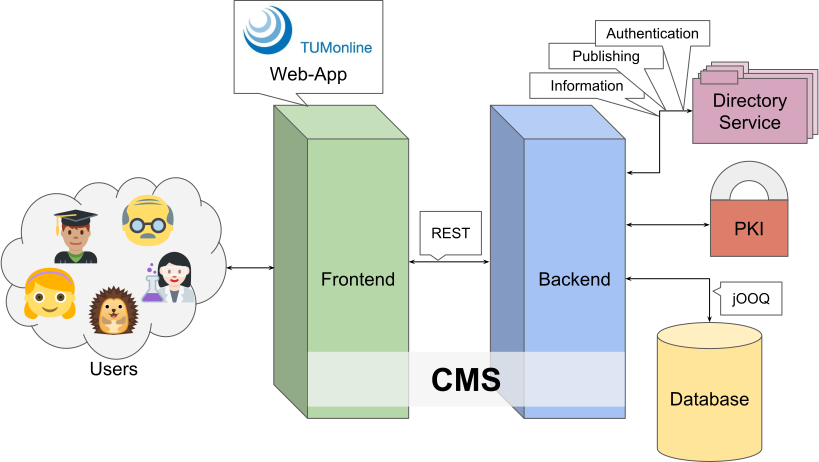
\includegraphics[width=.8\textwidth]{figures/systemArchitecture.pdf}
    \caption{Architecture of the certificate management system, based on the work of \citet{jagdish2016certservice}}
    \label{fig:systemArchitecture}
\end{figure}

The basic architecture of our system was proposed by \citet{jagdish2016certservice} in 2016.
Our system is very similar, with only slight adjustments to the architecture, as displayed in
\Cref{fig:systemArchitecture}.
The main differences between the proposed and implemented system are, that he identity management, authentication,
keyserver, and public key publishing components are not separated.
Although separate systems for those components should work in theory, most organizations handle all those tasks via a
single directory service as an identity management system.

In our approach, a web application handles the user interaction in a nice and user friendly way.
This webapp can be provided by familiar user interfaces, such as TUMonline in case of our university.
The app then in turn communicates via a REST interface with the certification management system as backend, which can
handle the certification components.

\section{User Centric features}\label{sec:userDetails}
The main ingredient of a certificate is authenticated information about users.
This information is then stored in the certificate, as detailed in \Cref{sec:publicKeyInfrastructure}.
Traditionally, users would generate the CSR themselves and the CA would only validate those fields.
From a user centric perspective, this is not ideal.
Since the CMS already knows this information, it should tell authenticated clients, which information it accepts as
authenticated.

Most of this information is readily available in organizations via an identity management system, which already serves
as authentication backend.
Most institutions have exhaustively verified users identities, so those systems can be used as fundamental basis of
authenticity.
Therefore, we automatically fetch personal information and trusted email addresses, while only requiring a single
authentication step.
With combined user authentication and information providers, the user experience should be as good as possible, since
manual intervention is reduced to a minimum.

Another problem is, that users usually struggle to properly back up their private key, or to securely transfer it to
other systems.
We therefore also provide a secure way to backup users' certificates, since easy access to their certificates is
essential to provide a good user experience.

\section{Integration Into Existing Systems}\label{sec:integrationIntoExistingSystems}
User friendliness is not only a design goal of the frontend, but also the backend APIs, that are documented and can be
used intuitively.
Reduction of setup, deployment and development complexity, results in a intuitive for administrators and future
extensions of the system.

Another important factor is the usage of industry standard tools, such as Java enterprise application.
Java enterprise servers are often already available in organizations, but can also easily be set up separately.
Different databases in organizations, provide abstraction from concrete database.

To implement a generic database connection we decided to use an Object Relational Mapper (ORM), that works with any
database an organization wishes to use.
Previously only MySQL was supported, a more generalized approach would be better, e.g.\ to store data in an Oracle
database, such as TUM uses for its TUMonline.

Furthermore, mismatches between database schema and Java objects are only detected during runtime, which increases
testing overhead.
This can be statically checked at compile time, which should decrease bugs and increase developer productivity

\section{Compatibility With Embedded Devices}\label{sec:compatibilityWithEmbeddedDevices}
With the rise of the Internet of Things (IoT), many appliances have a need to communicate with users and each other.
To also provide certificates to those devices, we envision complete hands-off provisioning of certificates on embedded
devices.
To enable those applications, we design our solution to be fully scriptable, complete with generation and distribution
of certificates.
This essentially boils down to providing an API, which can be universally used.
Such APIs are commonly designed as Representational State Transfer (REST) systems, which we decided to use.

\section{Certificate Exchange}\label{sec:certificateExchange}
One of the main features for PKI (c.f.~\ref{sec:publicKeyInfrastructure}), the Certificate Repository also needs to be
added, such that certificates can be published in a more generic way.
To implement such a repository, there are several different methods, as detailed by
\citet{hauner2016interoperability}:
One possibility would be to publish the certificates via the Lightweight Directory Access Protocol (LDAP).
The specification in RFC4523~\cite{RFC4523} defines the \lstinline{userCertificate} field for X.509 Certificates.

An alternative would be DNS-Based Authentication of Named Entities (DANE), as defined in RFC8162~\cite{RFC8162} via the
SMIMEA DNS record.
Similar to that approach, OpenPGP certificates can also be published using DANE, as defined in RFC7929~\cite{RFC7929}.
However in this work, we will only concentrate on on X.509 certificates.
Additionally, we provide the foundations to future extensions to support OpePGP\@.

Since there are two competing options in this case, we decided to only concentrate on the most widespread and accessible
option in organizations: LDAP\@.
LDAP servers are almost universally available, since most user authentication systems are based on it, most famously
Microsoft's Active Directory.
